% !TEX root = Skin_Lesion_Classification_Using_Machine_Learning.tex

% #TODO this is very long, check for redundant parts

\section{Skin Classification using Convolutional Neural Network and Metadata [HBT]}\label{sec:metadata_cnn}
The Neural Networks with multiple inputs when the network require data from multiple sources or in different formats. For example, networks that require image data captured from multiple sensors at different resolutions. In many researches, the use of different type of data along with the image data for classification in deep learning has shown the considerable improvement in image classification\cite{love},\cite{melan}. The metadata is merged within the same pixel matrix of the image in each RGB layer which enriches the extraction of features, has shown significant improvement in accuracy in this research\cite{melan}. The image metadata is used nonparametrically to generate neighbourhoods of related images using Jaccard similarities, then used a deep neural network to blend visual information from the image and its neighbours in this research \cite{love}. McAuley and Leskovec pioneered the study of multilabel image annotation using metadata, and demonstrated impressive results using only metadata. In hope of improvement of accuracy mixed data approach is used.
\subsection{Data Pre-processing and Data loading [HBT]}
The meta data which is numerical data consists of age, gender and the position of the skin lesion on the patient’s body. The sex data is one-hot encoded like female as 1, male as 0 and empty spaces as 3, to improve the data pre-processing step. The age data is already numerical value, so it is taken without one hot encoding. The loading of csv files into data frame and processed. The image data splitting is performed by customised function, where the whole image data is splitting into training data and testing data. The meta data is also splitting using the same function with respect to image data and mapping of metadata to corresponding image data is performed by using image file name. The listed pre-processing tasks are performed using Pandas library.

Even though the Keras API is capable of handling higher resolution images as input, the use of OpenCV library provides few computational problems to handle the high-resolution images. The larger image dataset is handled by resizing the images. So smaller resolution images are given as input to the CNN model. The use of OpenCV library functions to load images and original images are very large, so resized the image to desired size i.e,224 x 224 x 3. The image data is converted to NumPy array format for easy computation. Normalization is done to scale the values to have a similar data distribution and nullify the effect of large values. Since the model is handling two different types of data, which requires separate pre-processing steps including scaling, normalization, and feature engineering. This is extremely challenge encountered in recent researches.
\subsection{Multi-Input Model Architecture [HBT]}
\begin{figure}[h]
    \centering
    % include first image
    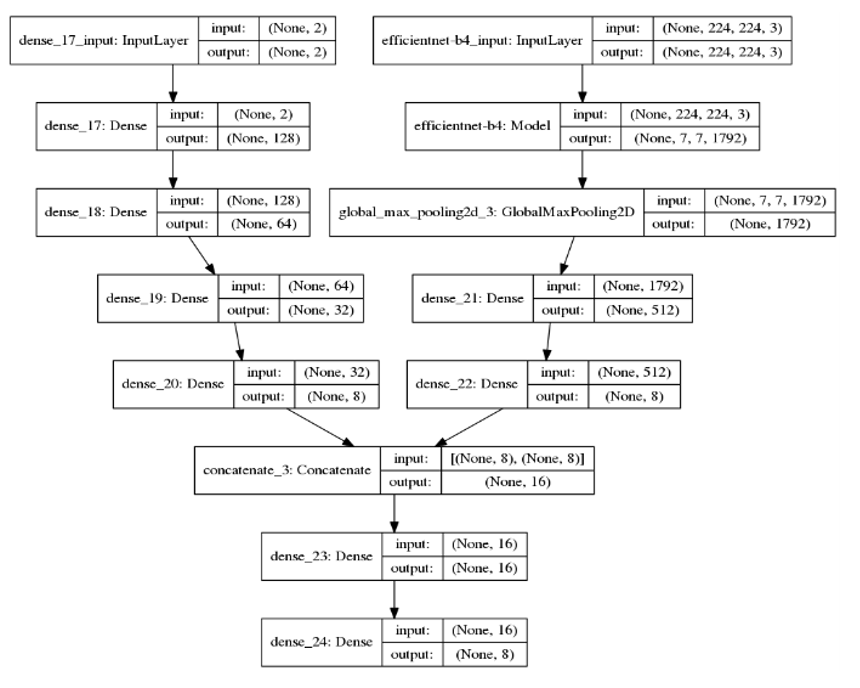
\includegraphics[width=.75\linewidth]{pictures/model.PNG}  
    \caption{Multi - Input model that includes both CNN and MLP branches to handle mixed data.}
    \label{fig:model}
\end{figure}
% #TODO this picture is way to small to read
The multi-input model is built to handle both image input and metadata which is a numerical data input is challenging task. The Keras API is used to build the multi input model, there is a requirement of two branches. First branch is a Multi-Layer Perceptron (MLP) model is designed to handle metadata and second branch is Convolution Neural Networks (CNN) for image data. Finally, these two branches are concatenated to have final model for training. The process of scaling is random in conventional CNN and is proved not be efficient. The reuse of scaling technique along single dimension alone can improve the accuracy, but model will quickly saturate\cite{tan2019efficientnet}. The transfer learning is performed to save computational time by a pre-trained CNN model EfficientNet, which involves systematic and principled scaling of depth, width and Resolution performs better than all the existing deep learning networks used in CNN \cite{tan2019efficientnet}.
MLP model consists of 4 layers with relu activation function with (128,64,32,8) neurons respectively. With 2 inputs age and sex respectively.The conventional customised CNN model with 3 layers, with 3x3 filter size and (16,32,64) depth respectively and stride of 2 is chosen. Padding is done to the images to maintain the same length. Another CNN model with EfficientNet B4 for transfer learning followed by GlobalMaxPooling and 2 Dense layers with (512,8) neurons with SoftMax activation to the pretrained network. The transfer learning is performed using both the EfficientNet model and conventional CNN for better approximation of expected outputs. 
\subsection{Training[HBT]}
The model is trained on a Nvidia Tesla P100 with 16GB of video memory via Google Colab. The model is developed using Keras API. We combined the MLP and CNN model using Concatenate function from Keras API to combine these two sub models. Now for final we provide the processed meta data as well as normalized image data array. The model compilation uses ‘Adam’ as optimizer and ‘accuracy’ as metric. The multi-class classification requires ‘categorical\_crossentropy’ as loss function. 
Training is done with image of 224 of height,224 of width, for 30 epochs and batch size of 32. In case of CNN with transfer learning, last 125 layers are unfreezed and fine-tuned them to be trainable to fit for our classification model and observe specific features related the image data given. First few layers of CNN are freezed to make them learn abstract features like edges, contours and many more features.

\subsection{Learning and conclusion}

Training accuracy of 54.52\% and Validation accuracy of 53.63\% was achieved using Multi-Input model. There is huge requirement of improvement in image data pre-processing techniques, hyper-parameter tuning, extracting features from image related to metadata for multi-input model as compared CNN model by considering only image data. Since the images are loaded using Open CV at onetime without using any Data Loading Pipeline, the training was taking very long time for each epoch. Normalizing is done at once for a whole image array is not efficient way and proved by experimenting it. 
 The accuracy is better for CNN model with a pre-trained EfficientNet model. Since the computational problems caused by OpenCV library in high resolution image data loading as input to multi-input model requires implementation of precise image processing techniques and a precise regularization with the loss obtained from model. The learning has to be regulated by considering metadata with respect to image data. Image augmentation and few other techniques may enhance the accuracy.  


